% =====================================================================
% WOWERS Master's Thesis — Mohamed's working file (Track M drafts)
% ---------------------------------------------------------------------
% This is NOT the master document — thesis_tom.tex is. This file exists so
% Mohamed can draft and compile the frontend sections (M1, M2) in isolation,
% without touching Tom's file or fighting over merge conflicts on a single
% 2,900-line document.
%
% At combine time (after both M1 and M2 have a first draft), copy the body
% prose from the two sections below verbatim into thesis_tom.tex, replacing
% the matching \wptodo stub:
%   - M1 → replaces the \wptodo at "\section{Frontend Visualization System}"
%     (currently thesis_tom.tex line ~1915, end of Chapter 4)
%   - M2 → replaces the \wptodo at "\subsection{Frontend Performance}"
%     (currently thesis_tom.tex line ~2281, inside Chapter 5)
%
% The preamble below is copied from thesis_tom.tex so this file compiles
% standalone with the same look (12pt, double-spaced body, same helper
% commands). Section/figure/table NUMBERS here will NOT match the final
% numbering in thesis_tom.tex — that only happens after the paste, when
% the sequential figure/table counters run across the whole document.
%
% WORKFLOW (see thesis/THESIS_BREAKDOWN.md):
%   - One work package at a time: draft M1 fully, stop, log the session in
%     THESIS_JOURNAL.md and tick it in THESIS_BREAKDOWN.md, THEN start M2.
%   - Obey thesis/thesis_format_prompt.md (voice, numbers, honesty, fig/tab
%     rules) — same rules Tom's chapters follow.
%   - Never cite this repo's own .md files (journal, reports, prompts). Any
%     claim needing a citation traces to an external source (paper, vendor
%     doc, dataset, standard) — see THESIS_BREAKDOWN.md's RULE at the top.
%   - Figures that must be real rendered images: produce them (screenshot /
%     script) and embed, or ask the user and leave a \figpending marker.
%     Never fabricate or leave a silent blank.
%
% COMPILE:  pdflatex thesis_moh.tex   (run twice for TOC/refs)
% =====================================================================
\documentclass[12pt,letterpaper]{report}

\usepackage[left=1.5in,right=1in,top=1in,bottom=1in]{geometry}
\usepackage{setspace}
\doublespacing
\usepackage{graphicx}
\usepackage{booktabs}
\usepackage{amsmath}
\usepackage{caption}
\usepackage{etoolbox}
\usepackage{tocloft}

\captionsetup{font=singlespacing}
\AtBeginEnvironment{tabular}{\singlespacing}
\AtBeginEnvironment{thebibliography}{\singlespacing\setlength{\itemsep}{0.6em}}
\usepackage[hidelinks]{hyperref}
\usepackage{xcolor}
% tikz is used locally for the M1 application-flow diagram (Figure below).
% thesis_tom.tex dropped tikz in favor of drawio-exported assets for its own
% figures (see THESIS_JOURNAL.md, 2026-07-24 session) -- decide at J5 combine
% time whether to keep this one as TikZ or re-author it in drawio to match.
\usepackage{tikz}
\usetikzlibrary{arrows.meta,positioning,fit}

\usepackage{longtable}
\AtBeginEnvironment{longtable}{\singlespacing}
\usepackage{chngcntr}
\counterwithout{figure}{chapter}
\counterwithout{table}{chapter}

\renewcommand{\cftchapleader}{\cftdotfill{\cftdotsep}}
\renewcommand{\cftchapfont}{\normalfont\bfseries}
\renewcommand{\cftchappagefont}{\normalfont\bfseries}

% --- helper: placeholder for a not-yet-written work package -----------
\newcommand{\wptodo}[2]{%
  \par\medskip\noindent\textcolor{red}{\textbf{[TODO — #1]}}\ \textit{#2}\par\medskip}

% --- helper: figure pending upload (per THESIS_BREAKDOWN images rule) ---
\newcommand{\figpending}[3]{%
  \begin{figure}[htbp]\centering
    \fbox{\parbox{0.85\linewidth}{\centering\vspace{1.5em}%
      \textbf{[FIGURE #1 PENDING --- awaiting upload: #2]}%
      \vspace{1.5em}}}
    \caption{#3}\label{fig:#1}
  \end{figure}}

\title{WOWERS Thesis --- Mohamed's Working File (Track M)}
\author{Mohamed Abdel Hamid}
\date{}

\begin{document}
\pagenumbering{arabic}
\tableofcontents
\clearpage

% =====================================================================
% M1 · Chapter 4.6 — Frontend Visualization System (~2,000 w)
% Final position in thesis_tom.tex: end of Chapter 4 (Design Details),
% as \section{Frontend Visualization System}.
% =====================================================================
\chapter{[Draft only — merges into Ch.\ 4] Frontend Visualization System}

The screening pipeline described in the preceding sections of Chapter 4 ends
at a single deterministic data contract, the 58-property GeoJSON file
exported by \texttt{export\_geojson.py}. That file is inert on its own: it
is the frontend's responsibility to turn it into a tool a non-technical
reviewer, an investor, or a municipal utility can actually use to find and
evaluate a candidate site. Concretely, the frontend renders every scored
plant on an interactive national map, lets a user narrow that set by state,
turbine type, payback period, and data-quality tier, and drills from any
site down to a full financial and physical scorecard. It runs entirely as a
static single-page application (SPA): there is no server process, no
database, and no API behind it, a constraint that follows directly from the
export layer's own design and is not an independent decision. How that
constraint shaped the stack, the data layer, and the view architecture will
now be discussed.

\section{Stack Selection}

Three architectures were considered for turning the exported GeoJSON into a
usable tool. The first was a server-rendered dashboard, a small Python
backend (Flask or FastAPI) that queries the parquets or the GeoJSON file on
every request and renders HTML server-side. The second was a
notebook-style analytics app, Streamlit or Dash, which trades custom UI
control for fast iteration on data-heavy views. The third was a static
single-page application that fetches one pre-exported file once and does
all filtering, sorting, and view derivation in the browser. The static SPA
was chosen because the pipeline's output is already a batch artifact,
regenerated on demand rather than on every request, so a server that
re-queries it for each page load adds operational surface (a process to
keep running, a host to pay for) without adding any capability the static
file cannot already provide. This also matches how the export layer itself
was designed, byte-deterministic and git-tracked so that the exact file a
browser fetches is the exact file reviewed and committed, with no server-side
state that could drift from it.

Within that choice, three further decisions had to be made. For the
application framework, React 19.2~\cite{react19} was chosen over a
framework-free approach or Vue, because the view set (seven distinct routed
pages sharing a common data layer and a consistent set of formatting and
color-coding rules) is naturally expressed as a small component tree, and
React's ecosystem includes typed, actively maintained bindings for both of
the remaining two decisions. TypeScript~5.7~\cite{typescript} was used
throughout rather than plain JavaScript so that the 58-property data
contract could be declared once, in \texttt{lib/types.ts}, and checked at
build time everywhere it is consumed; a property renamed or dropped in the
exporter surfaces as a compile error in the frontend rather than a silent
\texttt{undefined} on a live dashboard. The build tool is
Vite~7.1~\cite{vite7}, chosen over Create React App or webpack directly for
its native ES module dev server and its \texttt{?url} asset-import syntax,
which is what lets the GeoJSON file be imported as a versioned, hashed
static asset (see Section~4.6.2) instead of being fetched from a hand-built
path.

For the map layer, three libraries were considered: Leaflet with raster
tile layers, Mapbox GL~JS, and MapLibre GL~JS. Leaflet was set aside because
its DOM/SVG-based marker rendering does not scale cleanly to the full
3{,}778-site scored set at national zoom. Mapbox GL was set aside because it
requires a paid API token for both tiles and the GL runtime itself, an
ongoing operating cost and an external dependency this project's
non-technical stakeholders should not have to manage. MapLibre
GL~JS~5.1~\cite{maplibregl}, an open-source, token-free fork of Mapbox GL~JS
v1, was chosen instead: it renders point data as a single WebGL circle layer
regardless of point count, and it is wrapped through
\texttt{react-map-gl}~8.0~\cite{reactmapgl} so the map is expressed
declaratively as \texttt{<Map>}, \texttt{<Source>}, and \texttt{<Layer>}
components rather than through imperative MapLibre calls scattered across
component lifecycle hooks.

For charting, hand-rolled SVG (or a lower-level library such as D3 directly)
and Chart.js were considered against Recharts~3.0~\cite{recharts3}.
Recharts was chosen because its composable, React-native component API
(\texttt{<BarChart>}, \texttt{<ScatterChart>}, \texttt{<AreaChart>}) matches
the rest of the codebase's component style and needed no imperative canvas
management. One chart does not use Recharts: the capacity-factor gauge on
the plant detail page is custom inline SVG, built in \texttt{Gauge.tsx},
because Recharts has no radial-needle gauge primitive, and the display this
project needed, a needle fixed to capacity factor on a 0--100\% scale with
P10/P50/P90 energy figures labeled beneath it, was simpler to draw directly
as an SVG arc than to bend a general-purpose charting library toward it.

\section{Data Layer and View Architecture}

The frontend went through two data-layer designs before reaching its
current form. The first, built alongside the initial three-view dashboard,
used a 308-line Python exporter that read the four production parquets and
wrote four separate artifacts under \texttt{frontend/public/data/}: a slim
map GeoJSON, a national KPI summary, one portfolio file per state, and one
detail file per plant. That design required a Python step before every
\texttt{npm run dev}, and it duplicated, in a second file format, exactly
the join logic already implemented in the export layer described in
Section~4.5. It was replaced the same day by the design the frontend uses
today: the single git-tracked \texttt{exports/scored\_sites.geojson}, the
same 58-property, 3{,}778-feature file described in Section~4.5, is the
frontend's only data source.

\texttt{lib/data.ts} implements this as a module-level cached fetch.
\texttt{sitesUrl} is a Vite \texttt{?url} import of the GeoJSON file one
directory above the frontend package, so the exact file a build embeds is
the exact file tracked in the repository, with no copy step and no
possibility of the two drifting. The first call to \texttt{loadSites()}
issues one \texttt{fetch()} and stores the pending promise; every
subsequent call across every view returns that same cached promise rather
than re-fetching, so navigating between the seven routes costs one network
request for the life of the session. A local \texttt{SiteProps} interface
mirrors the exporter's 58 properties field for field, and four exported
functions, \texttt{fetchPlants}, \texttt{fetchNational},
\texttt{fetchPortfolio(state)}, and \texttt{fetchPlant(id)}, derive the four
view-specific shapes the components consume entirely in the browser. This
client-side derivation reproduces classification rules that previously
lived in the Python exporter: \texttt{payback()} treats any value at or
above $10^5$ as the pipeline's ``never pays back'' sentinel and rounds the
remainder to two decimal places \emph{before} banding, because the export
layer's own rounding happens before its banding and a boundary value such
as 4.9996~yr bands as ``high'' (\textless 5~yr) on the raw figure but
``moderate'' on the rounded one; \texttt{viabilityBand()} then bins that
rounded payback into the four legend categories shown on every map and
table (high \textless 5~yr, moderate 5--15~yr, marginal 15--20~yr,
non-viable otherwise); and \texttt{siteConfidence()} maps the exporter's
\texttt{data\_quality} and \texttt{project\_viable\_high\_confidence}
fields onto a three-level High/Medium/Lower badge shown throughout the
interface.

Seven routes are declared in \texttt{App.tsx} using React Router~7. The
root route, \texttt{NationalMap}, is the landing view: a MapLibre map of
every scored site colored by viability band, a left filter panel (state,
turbine type including an explicit ``Unassigned'' bucket, a 1--20~yr payback
slider where the maximum setting removes the payback filter entirely rather
than clamping at 20, and a high-confidence-only toggle), header KPI tiles
recomputed live from the currently filtered feature set rather than from a
static national total, and a right-hand panel listing the top five
opportunities by NPV plus a bar chart of viable sites by state.
\texttt{/state/:code} (\texttt{StatePortfolio}) shows every scored site in
one state as a sortable, paginated, CSV-exportable table alongside an
energy bar chart of the top ten sites and a payback-versus-NPV risk/return
scatter. \texttt{/plant/:id} (\texttt{PlantDetail}) is the single-site
view: a three-column layout presenting flow data, elevation data, and a
satellite mini-map on the left; the energy-recovery gauge and a recommended
turbine card with a synthesized efficiency curve in the center; and a
financial scorecard, a sensitivity tornado chart, and outbound
next-step links (a per-turbine-type manufacturer page, the DOE Water Power
Technologies Office funding page, and a link to similar sites filtered by
the same state and turbine type) on the right. \texttt{/opportunities} and
\texttt{/plants} both reuse a single shared \texttt{SiteTable} component,
pre-filtered to \texttt{project\_viable} sites in the first case and
unfiltered across all 3{,}778 scored sites in the second, each with its own
URL-parameter filters so either can serve as a deep-link target from
another view. \texttt{/analytics} aggregates the whole portfolio into a
payback-distribution histogram, a per-state bar, a turbine-mix bar, and a
combined viability-band and confidence-tier breakdown. \texttt{/reports}
presents the national summary as a plain key-value grid alongside one-click
CSV downloads (all sites, viable sites only, and a state summary) and a
short data-sources note. A wildcard route redirects any unmatched path back
to the root. Figure~\ref{fig:m1-flow} shows this structure: every routed
view calls into the same four \texttt{lib/data.ts} functions, and every one
of those functions is served from the single cached fetch of
\texttt{scored\_sites.geojson}.

\begin{figure}[htbp]\centering
\resizebox{\linewidth}{!}{%
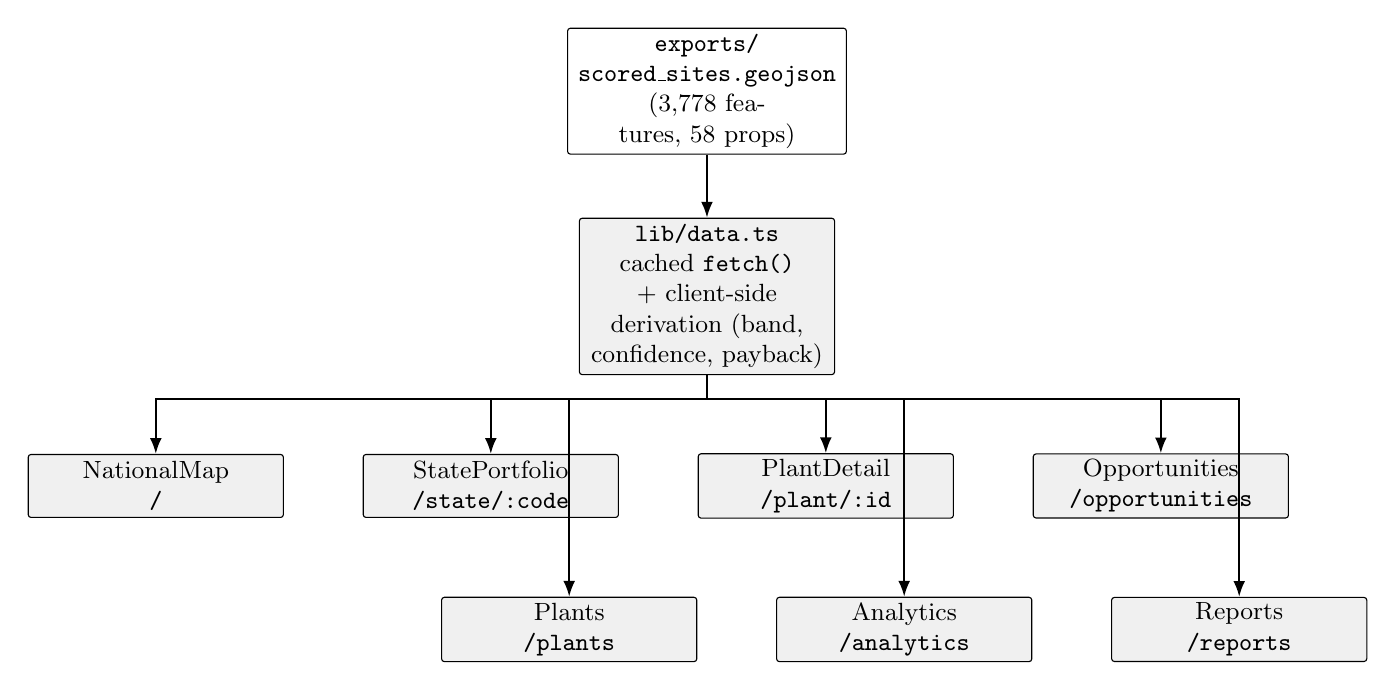
\begin{tikzpicture}[
  node distance=8mm and 10mm,
  box/.style={draw=black, fill=gray!12, rounded corners=1pt, align=center,
              font=\small, minimum height=8mm, text width=31mm, inner sep=2pt},
  src/.style={draw=black, fill=white, rounded corners=1pt, align=center,
              font=\small, minimum height=8mm, text width=34mm, inner sep=2pt},
  arr/.style={-{Latex[length=2mm]}, thick}
]
\node[src] (geo) {\texttt{exports/}\\\texttt{scored\_sites.geojson}\\(3{,}778 features, 58 props)};
\node[box, below=of geo] (data) {\texttt{lib/data.ts}\\cached \texttt{fetch()} + client-side\\derivation (band, confidence, payback)};
\node[box, below=10mm of data, xshift=-70mm] (v1) {NationalMap\\\texttt{/}};
\node[box, right=of v1] (v2) {StatePortfolio\\\texttt{/state/:code}};
\node[box, right=of v2] (v3) {PlantDetail\\\texttt{/plant/:id}};
\node[box, right=of v3] (v4) {Opportunities\\\texttt{/opportunities}};
\node[box, below=10mm of v1, xshift=52.5mm] (v5) {Plants\\\texttt{/plants}};
\node[box, right=of v5] (v6) {Analytics\\\texttt{/analytics}};
\node[box, right=of v6] (v7) {Reports\\\texttt{/reports}};
\draw[arr] (geo) -- (data);
\draw[arr] (data.south) -- ++(0,-3mm) -| (v1.north);
\draw[arr] (data.south) -- ++(0,-3mm) -| (v2.north);
\draw[arr] (data.south) -- ++(0,-3mm) -| (v3.north);
\draw[arr] (data.south) -- ++(0,-3mm) -| (v4.north);
\draw[arr] (data.south) -- ++(0,-3mm) -| (v5.north);
\draw[arr] (data.south) -- ++(0,-3mm) -| (v6.north);
\draw[arr] (data.south) -- ++(0,-3mm) -| (v7.north);
\end{tikzpicture}%
}
\caption{Frontend application flow: seven React Router views all resolve
through the same four \texttt{lib/data.ts} functions, backed by one cached
fetch of the single tracked GeoJSON file}
\label{fig:m1-flow}
\end{figure}

\figpending{m1-nationalmap}{a live screenshot of the National Opportunity
Map view (route \texttt{/}) --- run \texttt{npm run dev} in
\texttt{frontend/} and screenshot the browser at
\texttt{http://localhost:5173/}. Verified live this session: the map
renders 3{,}778 sites colored by band, header KPIs read 3{,}778 sites shown
/ 1{,}138 viable / \$310.1M NPV / 9.8~yr median payback at the default
(unfiltered) state, matching the P2-SEED baseline exactly.}{National
Opportunity Map view}

\figpending{m1-plantdetail}{a live screenshot of a Plant Detail view
(route \texttt{/plant/:id}) --- run \texttt{npm run dev} in
\texttt{frontend/} and screenshot, e.g., \texttt{http://localhost:5173/}
\texttt{plant/OH0024732}. Verified live this session: flow, elevation,
gauge, turbine, financial scorecard, and sensitivity tornado all populate
correctly from the geojson.}{Plant Detail view}

\section{Interaction, Filtering, and Export}

Two shared conventions run across every filterable view. First, filter
state lives in the URL query string via React Router's
\texttt{useSearchParams}, not in component state: \texttt{NationalMap}
encodes state, turbine-type list, maximum payback, and the high-confidence
toggle as \texttt{?state=\&turb=\&pb=\&hc=}, and \texttt{Plants} does the
same for its own filter set. A filtered view is therefore a shareable,
bookmarkable, refresh-safe link rather than transient client state, and it
is also how one view deep-links into another, for example the ``View
Similar Sites'' action on the plant detail page, which links to
\texttt{/plants} pre-filtered to the same state and turbine type. Second,
every table (\texttt{SiteTable}, used by both \texttt{Opportunities} and
\texttt{Plants}, and the portfolio table in \texttt{StatePortfolio}) is
independently sortable by column, searchable by name, city, state, or
NPDES~ID, paginated at 50 rows per page, and exportable to CSV through a
shared \texttt{downloadCsv} helper that builds the file as a
\texttt{Blob} in the browser and triggers a download with no server round
trip.

On the map itself, clicking any point navigates to that site's detail
page; hovering shows a popup with name, location, energy, payback, and
NPV. Selecting a state from the filter panel calls MapLibre's
\texttt{fitBounds} against the minimum and maximum longitude and latitude
of that state's features, easing the view to it; this call is gated on the
map's \texttt{onLoad} event, because an earlier version fired
\texttt{fitBounds} before the underlying map instance existed whenever a
state was present in the URL on first page load, a race that silently
failed to zoom on a fresh deep link. A basemap toggle switches between two
token-free raster sources, CARTO Positron for a light reference map and
Esri World Imagery for satellite, drawn as a two-button control over the
map canvas; the same satellite style is reused, at a fixed close zoom, for
the small locator map on the plant detail page.

\section{Limitations}

Five limitations are named. First, the initial page load fetches the
entire 6.13~MB scored-sites file regardless of which view is opened, the
same whole-file cost noted from the export side in Section~4.5; this is
acceptable at 3{,}778 sites but would need a change, most likely a
tiled or paginated data endpoint, if the screened fleet grew by an order of
magnitude. Second, the production JavaScript bundle is not code-split by
route, so the MapLibre GL runtime is downloaded even when a user opens
\texttt{/reports} and never touches the map; route-level lazy loading
(React's \texttt{lazy()}) would defer that cost to the views that need it
and is the named fix, not yet built. Third, the national map draws every
point individually with no clustering, so dense regions such as the
Northeast corridor overplot at the default national zoom; the per-state
zoom-to-bounds interaction mitigates this once a state is selected but does
not address the initial national view, and marker clustering at low zoom is
the deferred fix. Fourth, every filter, sort, search, and pagination
operation runs client-side over the full in-memory feature array; this
costs nothing perceptible at 3{,}778 features but is a ceiling that would
require server-side query support to lift. Fifth, the efficiency curve
drawn on the plant detail page is a synthesized unimodal approximation
centered on each turbine's rated flow and peak efficiency, not a measured
or vendor-published per-unit curve; it exists to make the recommended
turbine's operating envelope legible at a glance and should not be read as
an engineering specification. A sixth item is procedural rather than
architectural and is worth recording here: the manufacturer links surfaced
on the plant detail page (one vendor per recommended turbine type) are
representative suppliers chosen for the demonstration, not endorsements or
confirmed live quotes, and should be re-verified before any external use of
the dashboard. The frontend's measured build and quality-assurance results
are reported next, in Section~5.1.6.

% =====================================================================
% M2 · Chapter 5.1.6 — Frontend Performance (~700 w)
% Final position in thesis_tom.tex: inside Chapter 5 (Experiments and
% Results), as \subsection{Frontend Performance}, immediately before the
% System Integration Test (J4).
% =====================================================================
% ---------------------------------------------------------------------
% Local reference list for Track M citations used above. At J5 combine
% time these \bibitem entries move into thesis_tom.tex's single
% \begin{thebibliography}; none of these keys currently collide with
% Tom's existing keys (checked against thesis_tom.tex 2026-07-29).
% ---------------------------------------------------------------------
\begin{thebibliography}{99}

\bibitem{react19}
Meta Platforms, Inc. and the React community,
``React --- The Library for Web and Native User Interfaces,'' version 19.2,
2025. [Online]. Available: https://react.dev/.
[Accessed 29 Jul.\ 2026].

\bibitem{typescript}
Microsoft Corporation,
``TypeScript,'' version 5.7, 2025.
[Online]. Available: https://www.typescriptlang.org/.
[Accessed 29 Jul.\ 2026].

\bibitem{vite7}
E.~You and the Vite community,
``Vite,'' version 7.1, 2025.
[Online]. Available: https://vite.dev/.
[Accessed 29 Jul.\ 2026].

\bibitem{maplibregl}
MapLibre contributors,
``MapLibre GL JS,'' version 5.1, 2025.
[Online]. Available: https://maplibre.org/maplibre-gl-js/docs/.
[Accessed 29 Jul.\ 2026].

\bibitem{reactmapgl}
visgl,
``react-map-gl,'' version 8.0, 2025.
[Online]. Available: https://visgl.github.io/react-map-gl/.
[Accessed 29 Jul.\ 2026].

\bibitem{recharts3}
Recharts Group,
``Recharts --- A Composable Charting Library Built on React Components,''
version 3.0, 2025.
[Online]. Available: https://recharts.org/.
[Accessed 29 Jul.\ 2026].

\end{thebibliography}

\chapter{[Draft only — merges into Ch.\ 5] Frontend Performance}

Every number in this section was measured this session, from a clean
build and a live browsing session against the dev server, rather than
carried over from an earlier note. This distinction matters here more than
in most results sections: the frontend is the one part of the platform
whose behavior can drift with the local toolchain (Node, npm, browser)
independently of any change to the WOWERS source itself, so a reused
figure would not actually be verifying anything.

\subsection*{Build Performance}

A clean build was run with \texttt{rm~-rf~dist~\&\&~npm~run~build} under
Node~22.11.0 and npm~11.6.1. The command runs \texttt{tsc~-b} before
\texttt{vite~build}, so a successful build is also a clean full-project
type-check: it passed with zero type errors before bundling began. Vite
7.3.5 then produced the bundle in 6.11~s. One environment finding is worth
recording plainly: Vite 7.3.5 reported that it requires Node.js~20.19+ or
22.12+, and 22.11.0 falls just short of the latter floor; the build still
completed without error, so this is a compatibility warning rather than a
failure, but it should be resolved before this frontend is built in any
automated or shared environment. Table~\ref{tab:m2-bundle} reports every
emitted asset.

\begin{table}[htbp]
\centering
\begin{tabular}{lrr}
\toprule
Asset & Raw size & Gzip size \\
\midrule
\texttt{index-*.js} (application code) & 711.33 kB & 214.71 kB \\
\texttt{maplibre-gl-*.js} (map runtime) & 1{,}053.37 kB & 284.75 kB \\
\texttt{index-*.css} & 75.06 kB & 11.61 kB \\
\texttt{scored\_sites-*.geojson} (data asset) & 6{,}129.14 kB & --- \\
\texttt{index.html} & 0.50 kB & 0.33 kB \\
\bottomrule
\end{tabular}
\caption{Production bundle sizes, measured this session from a clean \texttt{npm run build}}
\label{tab:m2-bundle}
\end{table}

Vite's own build output flags the two largest JavaScript chunks as
individually over its 500~kB warning threshold; that flag is the subject
of the discrepancy paragraph below. As a point of comparison, an earlier
project-journal note recorded a 2.6~s build and a 707~kB application
chunk from the same command; this session's 6.11~s and 711.33~kB are
close but not identical, which is expected of a build time and bundle
size measured on different hardware after further commits, and is not
treated as a regression.

\subsection*{Quality Assurance}

All seven routes (\texttt{/}, \texttt{/opportunities}, \texttt{/plants},
\texttt{/analytics}, \texttt{/reports}, one \texttt{/state/:code}, and one
\texttt{/plant/:id}) were exercised against the dev server this session.
Zero browser console errors and zero dev-server errors were observed
across all seven. Every headline figure checked against the P2-SEED
baseline matched exactly: the National Opportunity Map read 3{,}778 sites
shown, 1{,}138 viable, \$310.1M NPV, and a 9.8~yr median payback at its
default (unfiltered) state; Analytics read \$310.1M portfolio NPV,
\$211.3M CapEx, \$41.2M/yr savings, 409{,}170~MWh/yr recoverable energy,
and 848 high-confidence sites; Opportunities read 1{,}138 opportunities
and the same \$310.1M and 409{,}202~MWh/yr totals. The single-cached-fetch
design described in Section~4.6.2 was also confirmed empirically rather
than only by reading the source: after the initial page load, navigating
across four views through the in-app sidebar, a client-side transition
with no full page reload, produced zero additional network requests for
\texttt{scored\_sites.geojson}, matching the module-level cache's intended
behavior.

\subsection*{Discrepancy: Bundle Size and Deferred Code-Splitting}

The measured result departs from the ideal one in a specific, bounded way.
The gap: two chunks, the 711.33~kB application bundle and the
1{,}053.37~kB MapLibre runtime, are downloaded on every route, including
\texttt{/reports}, which never renders a map, for a combined 1{,}764.7~kB
raw (499.46~kB gzipped) of JavaScript the browser did not need for that
page. The mechanism: \texttt{App.tsx} imports all seven views statically,
and \texttt{MapView} is pulled in transitively through
\texttt{NationalMap} and through \texttt{PlantDetail}'s mini-map, so the
bundler has no route boundary at which it could separate the MapLibre
dependency into its own lazily loaded chunk. Whether this is acceptable
for the current scope: yes. At 499.46~kB gzipped total and a demonstration
audience of one reviewer at a time rather than concurrent production
traffic, the cost is a fraction of a second on any real connection, and it
was accepted as a known cost rather than an oversight in the
2026-07-07 session that first flagged it. The fix, not yet built, is
route-level code-splitting with React's \texttt{lazy()} so that the
MapLibre chunk is requested only when \texttt{NationalMap} or
\texttt{PlantDetail} is the active route. Map clustering at low zoom (see
the limitation named in Section~4.6.4) and a live backend to replace the
static GeoJSON fetch remain separately deferred and are not measured
here, because neither has been built in any form to measure.

\end{document}
